\chapter{Arquitetura Emocional Constru\'ida} \label{ch:aec}

\section{Visão Geral}

A presente arquitetura construída foi pensada conforme mostrado na
Figura~\ref{fig:vasc}. Como se pode observar, o sistema é dividido em um
ambiente e em agentes. O ambiente utiliza a ontologia de
rotinas para construir a visualização mostrada no capítulo~\ref{ch:cdu}.
Assim, o que o usuário vê é exibido a partir da descrição da ontologia de
rotinas. Mais detalhes ver seção~\ref{ch:aec:ocu}. Já a ontologia de preferências,
explicada na seção~\ref{ch:aec:oda}, permite guardar junto dos objetos do
mundo virtual informações e especificar como o ator é atraído por essas
informações.\dev{}

A segunda parte do sistema altera a mente dos atores agindo para acrescentar
anotações em suas percepções e para alterar o local que essas crenças são
salvas. A mente dos atores é chamada agente e eles recebem via percepção as suas
preferências e rotinas\dev{}. Essa escolha foi feita para permitir que a
escolha do que fazer seja toda ela escrita em código\dev{} da plataforma
\emph{Jason}. As emoções são concluídas pelo agente através de ontologia
(ver seção~\ref{ch:aec:omce}) e, portanto, a base de crenças padrão da
plataforma foi ampliada para consultar, guardar e recuperar as informações
diretamente da base de conhecimento quando a crença for relevante. Sendo
assim, é como se houvesse dois níveis. O primeiro formado pela ontologia e o
segundo pela base de crença padrão.

\begin{figure}
  \centering
  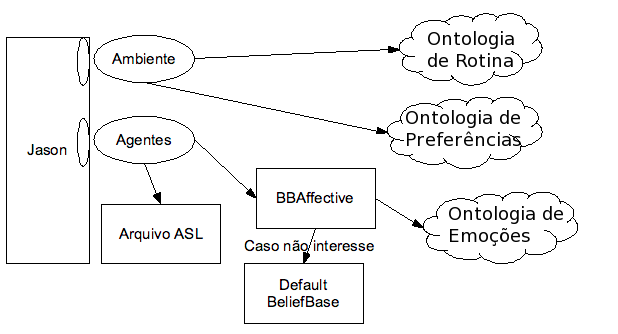
\includegraphics[width=10cm]{figuras/visao-geral.png}
  \caption{Visão abstrata do sistema construído.}
  \label{fig:vasc}
\end{figure}

\section{Ontologia do Modelo Cognitivo Emocional} \label{ch:aec:omce}

A fundamentação do modelo afetivo sendo utilizado aqui é o proposto por
\citet{ortony1988cse} e encontra-se explicado na seção \ref{ch-ca-mce}. A
ontologia proposta tinha como ideia inicial não utilizar regras, porém como
pode ser observado na Tabela~\ref{tab:oa:geral} foi necessário a criação de
regras para suportar o raciocínio no nível de indivíduo corretamente. As
regras que ajudam a conclusão das relações \emph{hasKnow}, \emph{hasFriend} e
\emph{hasEnemy} são diferentes das demais por causa que elas tem como
característica operar no domínio e na imagem da classe \emph{Agent}. Por
exemplo, se John avalia que se relaciona bem com Jose então John
\emph{hasFriend} Jose. Note que o contrario não é necessariamente verdade, o
Jose pode apenas saber que conhece o John então Jose \emph{hasKnow} John.

\begin{table}[h]
	\caption{Ontologia proposta com expressividade: ALCHIN(D).}
	\label{tab:oa:geral}
	\begin{center}
	\begin{tabular}{|c|c|}
	%\begin{tabular}{|p{34mm}|p{50mm}|p{50mm}|}
		\hline
		Descrição & Quantidade \\ \hline
		Classes &  45 		\\ \hline
		Propriedade de Objetos & 16 \\ \hline
		Propriedade de Dados & 14 \\ \hline
		Indivíduos &  0		\\ \hline
		Regras & 7 \\ \hline
	\end{tabular}
	\end{center}
\end{table}

Na Figura~\ref{fig:rlocc} são mostradas as regras desenvolvidas, elas dependem
que os indivíduos da ontologia sejam marcados como diferentes um dos outros.
Assim, recomenda-se fortemente que quando registrar um indivíduo da classe
\emph{Object} ou \emph{Agent} que a informação de igualdade ou diferenciação
seja preenchida\dev{}. Assim, se evita que o raciocinador conclua que não
conhece a resposta e chegue a uma conclusão não esperada.

\begin{figure}[b]
  \centering
  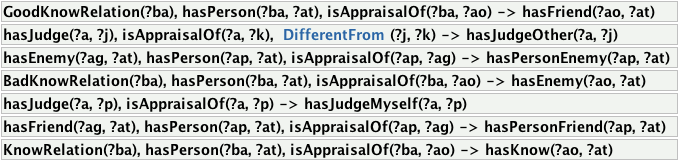
\includegraphics[width=14cm]{figuras/rules-LOCC.png}
  \caption{Regras da ontologia proposta.}
  \label{fig:rlocc}
\end{figure}

A Figura~\ref{fig:kplocc} mostra a árvore de relações que tem como imagem
dados ou instâncias (objetos). Ao se comparar as Figuras~\ref{fig:rlocc}
e \ref{fig:kplocc} se chega a conclusão que as propriedades que as
regras concluem não precisam ser configuradas pelo usuário. Assim, ao invés de
16 propriedades de objetos conforme informado na Tabela~\ref{tab:oa:geral}
apenas 9 precisam ser conhecidas. Dessas 9, a propriedade menos utilizada é a
\emph{hasSomething} que serve para indicar genericamente o que esta sendo avaliado. Note que
\emph{hasPerson} deve ser usado quando o indivíduo em avaliação for um membro
da classe \emph{Agent}. Já, a relação \emph{hasJudge} serve para indicar que o
membro da classe \emph{Object} esta sendo avaliado pela sua responsabilidade.
Por exemplo, Millie tem uma avaliação julgando seu carro com uma valoração
positiva.

\begin{figure}[b]
  \centering
  \begin{tabular}{cc}
  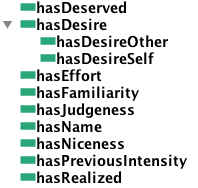
\includegraphics[height=4cm]{figuras/dataProperty-LOCC.png} & 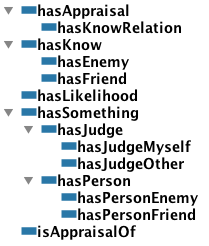
\includegraphics[height=5cm]{figuras/objectProperty-LOCC.png} \\
  (i) Relações de dados & (ii) Relações de Objetos
  \end{tabular}
  \caption{As relações existentes na ontologia proposta.}
  \label{fig:kplocc}
\end{figure}

Toda a valoração numérica existente na ontologia é inteira. Isso foi feito com a
finalidade de permitir que o usuário normalize\dev{} o número obtido da
maneira que desejar. Além disso, foi tomada a decisão de não especificar o
domínio da maioria das propriedades por causa que isso forçaria um
enquadramento em classes não desejadas. Por exemplo, se a relação
\emph{hasLikelihood} tiver o domínio \emph{ConsequenceForSelf} e existir um
indivíduo com somente essa relação então o mesmo seria enquadrado no conceito
\emph{ConsequenceForSelf}. Mas, o correto nesse caso seria não ser concluído nada,
ou seja, pertencer à classe \emph{Thing}.

A estrutura da ontologia pode ser visualizada na
Figura~\ref{fig:tlocc}~(pág.~\pageref{fig:tlocc}). Além disso, pode ser
recomendável olhar a
Figura~\ref{fig:occ_model}~(pág.~\pageref{fig:occ_model}) do modelo \occ
durante o resto da discussão dessa seção. Os sub-conceitos de \emph{Emotion}
correspondem aos três ramos do modelo original.
O ramo \emph{ActionsOfAgents} julga a responsabilidade e o quanto o agente que
realizou uma ação se desviou do esperado, o de
\emph{ConsequencesOfEvents} julga a consequência de um evento e
\emph{AspectsOfObjects} julga a atração para com um objeto.

O primeiro ramo a ser abordado é, o menos cognitivo, \emph{AspectsOfObjects}.
As emoções desse tipo são relacionadas com atratividade e familiaridade.
Entretanto, essas duas relações foram consideradas equivalentes porque o
importante, para o modelo, é quando ambas são positivas ou ambas negativas.
Assim sendo, uma pode assumir os dois papeis sem maiores penalidades e
simplificando a modelagem. A emoção \emph{Hate} é modelada como tendo a
propriedade de familiaridade (\emph{hasFamiliarity}) com valores negativos,
enquanto a emoção \emph{Love} tem valoração dessa mesma propriedade positiva.
Caso o valor seja zero, nada pode ser concluído.

Cabe notar que parece estranho uma emoção \emph{Love} com um objeto, porém
essa emoção foi escolhida por quem montou o modelo para representar seu tipo
por ser a mais forte de sua categoria. Assim, níveis menores implicam em
outros tipos de emoção. Além disso, agentes
podem ser vistos como objetos quando se esta avaliando a sua atração. Logo,
todo agente (\emph{Agent}) é um objeto (\emph{Object}). Por exemplo, John esta
apaixonado pela Millie (Millie é avaliada como objeto) ou John tem
repulsa por televisão.

O segundo conceito, chamado \emph{ActionsOfAgents}, pode ser pensado como
um ramo que julga a responsabilidade por uma determinada ação.
Assim, esse ramo é capaz de gerar emoções de: Admiração (\emph{Admiration}),
Orgulho (\emph{Pride}), Vergonha (\emph{Shame}) e Reprovação
(\emph{Reproach}). Por exemplo, Jose possui orgulho por cozinhar ou Dilu
reprova Jose porque ele come carne.

Na definição, as emoções de orgulho e vergonha podem acontecer mesmo quando se
esta avaliando ações de outras pessoas. Por exemplo, Dolores tem vergonha de
sua mãe que não cozinha. Essa conclusão é possível por causa de uma relação
que eles propõem de empatia\label{mark:empat}. Entretanto, como em nenhum outro momento, eles
dão mais detalhes sobre essa empatia foi resolvido considerar que vergonha e
orgulho são emoções sentidas somente quando o agente esta avaliando a si mesmo
e, dessa forma, o exemplo anterior não é possível no sistema desenvolvido. \dev{}
% dev -> poderia ter sido usado float e ter feito 1 (para si) e 0 (para outro)

As emoções que julgam responsabilidade são definidas como tendo uma relação de
julgamento (\emph{hasJudge}) e uma relação numérica que mapeia o valor
(\emph{hasJudgeness}) que representa o quanto o agente se desviou do
comportamento esperado, isto é, em casos de aprovação é um valor positivo e em
casos de reprovação é um valor negativo. Todavia, isso ainda não permite
diferenciar a emoção de admiração da emoção de orgulho ou a reprovação da de
vergonha. Essa distinção é possível ao se dividir a relação de julgamento com
duas sub-relações: tem auto-julgamento (\emph{hasJudgeMyself}) e tem
julgamento de outro (\emph{hasJudgeOther}).

A utilização de sub-propriedade torna possível escrever a ontologia da maneira
esperada suprimindo o problema. Entretanto, para o usuário pode se tornar
complicado ter que lembrar quando utilizar uma sub-propriedade ou outra.
Assim, foi resolvido deixar o usuário sempre utilizar a relação de julgamento
(\emph{hasJudge}) e via 2 regras inferir se é um auto-julgamento ou o
julgamento de outra pessoa. Para essas regras funcionarem da maneira correta,
o usuário deve declarar que os agentes ou objetos são diferentes uns dos
outros. Caso isso
não ocorra, o sistema considera que não há informação para verificar se um
indivíduo é igual ou diferente e conclui que não conhece a resposta. Além
disso, a relação de julgamento tem como imagem o conceito \emph{Object}.

Cabe salientar que toda avaliação tem pelo menos duas relações. A primeira
relação serve para conhecer quem esta avaliando (\emph{isAppraisalOf}) e a
seguinte serve para indicar quem ou o que esta sendo avaliado
(\emph{hasSomething}). Essa última pode não ser informada explicitamente porque pode
ser concluída quando usada uma de suas sub-relações. O último ramo, chamado de
\emph{ConsequencesOfEvents} é dividido em: \emph{ConsequencesForSelf} e
\emph{ConsequencesForOthers}. Toda essa divisão foca na consequência de um
evento realizado por algum agente. Por exemplo, Dilu tem pena
de Jose, Jose tem esperança de ser promovido, John tem satisfação por
estar almoçando ou Millie esta alegre por cozinhar.

\begin{wrapfigure}{r}{0.4\textwidth}
  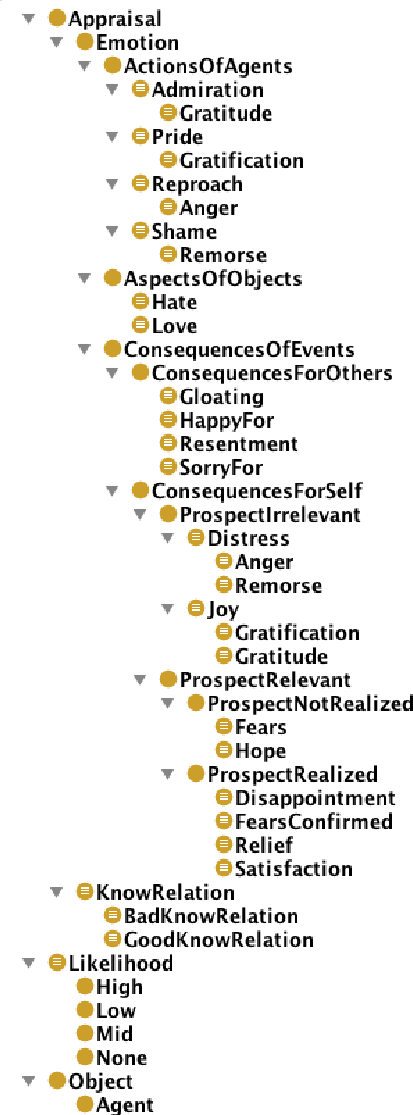
\includegraphics[height=149mm]{figuras/hierarquiaLOCC.png}
  \caption{Taxonomia da ontologia proposta baseado no modelo.}
  \label{fig:tlocc}
\end{wrapfigure}

A \emph{ConsequencesForOthers} expressa 4 emoções: \emph{Gloating},
\emph{HappyFor}, \emph{Resentment} e \emph{SorryFor}. Na definição, essas
emoções dependem: do grau de desejabilidade do avaliador para com o outro; do
grau de desejabilidade que se presume que o outro tenha; do grau de
merecimento do evento; e, do tipo de relacionamento com a pessoa. Na ontologia
proposta, a principal diferença com o modelo \occ é que foi considerado
que o grau de desejabilidade do avaliador para com o outro e o grau de
merecimento do evento são os mesmos. Dessa forma, se pode utilizar apenas três
relações para descrever as 4 emoções.

A relação de merecimento (\emph{hasDeserved}) e de desejabilidade
presumida (\emph{hasDesireOther}) são avaliadas de acordo com sua valoração
positiva ou negativa. Entretanto, a relação \emph{hasPerson} liga o outro indivíduo
sendo avaliado com a avaliação. Para se ter o conhecimento do que esta sendo julgado
ser amigo (\emph{GoodKnowRelation}) ou inimigo (\emph{BadKnowRelation}), esses
conceitos foram criados e precisam ser configurados para cada um dos agentes
em questão, porém quem precisa dessa informação é o conceito de avaliação
quando as relações \emph{hasPersonEnemy} e \emph{hasPersonFriend} precisam ser
descobertas. O agente pode declarar que só conhece uma pessoa, que conhece e é
um amigo ou que conhece e não gosta dela (inimiga).

\emph{ConsequencesForSelf} se divide entre consequências de eventos com
probabilidade (\emph{ProspectRelevant}) ou sem probabilidade
(\emph{ProspectIrrelevant}). Note que esses dois conceitos se
relacionam com probabilidade (\emph{hasLikelihood}). O primeiro conceito se
relaciona com a parte não nula, enquanto o outro se relaciona somente com
valores nulos. Dessa forma, ambos os conceitos são disjuntos. A classe com
probabilidade pode ser dividida ainda entre não
realizada (\emph{ProspectNotRealized}) e realizada (\emph{ProspectRealized}).

As emoções \emph{Fear} e \emph{Hope} fazem parte do conceito
\emph{ProspectNotRealized}. Esse conceito usa as relações \emph{hasLikelihood}
e \emph{hasDesireSelf}. Essa última é um número que
representa o desejo de se obter ou repudiar o evento. Além disso, quando o
evento ocorre a emoção atual pode virar uma emoção do conceito
\emph{ProspectRealized}, isto é, \emph{Fear} pode virar ou
\emph{FearsConfirmed} ou \emph{Relief} e \emph{Hope} pode virar ou
\emph{Satisfaction} ou \emph{Disappointment}.

\begin{table}[pt]
	\caption{Regras de classificação de indivíduos como emoções.}
	\label{table:lucca-emo}
	\begin{center}
	\begin{tabular}{|p{20mm}|p{120mm}|} % 140mm
		\hline
		Nome & Regra \\ \hline
		Fear & (hasLikelihood some (Likelihood and (not (None)))) and (hasDesireSelf some int[< "0" $\UP\UP$ int]) \\ \hline
		Hope & (hasLikelihood some (Likelihood and (not (None)))) and (hasDesireSelf some int[> "0" $\UP\UP$ int]) \\ \hline
		FearConfir-med & (hasEffort some int[< "0"$\UP\UP$int]) and (hasPreviousIntensity some int[< "0"$\UP\UP$int]) and (hasRealized some int[< "0"$\UP\UP$int]) \\ \hline
		Satisfaction & (hasEffort some int[> "0"$\UP\UP$int]) and (hasPreviousIntensity some int[> "0"$\UP\UP$int]) and (hasRealized some int[> "0"$\UP\UP$int]) \\ \hline
		Disappoint-ment & (hasEffort some int[> "0"$\UP\UP$int]) and (hasPreviousIntensity some int[> "0"$\UP\UP$int]) and (hasRealized some int[< "0"$\UP\UP$int]) \\ \hline
		Relief & (hasEffort some int[< "0"$\UP\UP$int]) and (hasPreviousIntensity some int[< "0"$\UP\UP$int]) and (hasRealized some int[> "0"$\UP\UP$int]) \\ \hline
		Gloating & (hasPersonEnemy some Agent) and (hasDeserved some int[> "0"$\UP\UP$int]) and (hasDesireOther some int[< "0"$\UP\UP$int]) \\ \hline
		HappyFor & (hasPersonFriend some Agent) and (hasDeserved some int[> "0"$\UP\UP$int]) and (hasDesireOther some int[> "0"$\UP\UP$int]) \\ \hline
		Resentment & (hasPersonEnemy some Agent) and (hasDeserved some int[< "0"$\UP\UP$int]) and (hasDesireOther some int[> "0"$\UP\UP$int]) \\ \hline
		SorryFor & (hasPersonFriend some Agent) and (hasDeserved some int[< "0"$\UP\UP$int]) and (hasDesireOther some int[< "0"$\UP\UP$int]) \\ \hline
		Distress & (hasLikelihood some None) and (hasDesireSelf some int[< "0"$\UP\UP$int]) \\ \hline
		Joy & (hasLikelihood some None) and (hasDesireSelf some int[> "0"$\UP\UP$int]) \\ \hline
		Hate & hasFamiliarity some int[< "0"$\UP\UP$int]\\ \hline
		Love & hasFamiliarity some int[> "0"$\UP\UP$int]\\ \hline
		Admiration & (hasJudgeOther some Object) and (hasJudgeness some int[> "0"$\UP\UP$int])\\ \hline
		Pride & (hasJudgeMyself some Object) and (hasJudgeness some int[> "0"$\UP\UP$int])\\ \hline
		Reproach & (hasJudgeOther some Object) and (hasJudgeness some int[< "0"$\UP\UP$int])\\ \hline
		Shame & (hasJudgeMyself some Object) and (hasJudgeness some int[< "0"$\UP\UP$int])\\ \hline
		Anger & Distress and Reproach \\ \hline
		Gratification &  Joy and Pride \\ \hline
		Gratitude & Joy and Admiration \\ \hline
		Remorse & Distress and Shame \\ \hline
	\end{tabular}
	\end{center}
\end{table}

O conceito \emph{ProspectRealized} não se relaciona em nenhum momento com a
relação \emph{hasLikelihood} porque o evento já aconteceu ou não vai mais
acontecer. Assim, ele possui três relações distintas das anteriores, a
primeira é o grau de realização do evento (\emph{hasRealized}), isto é, a
visão do agente sobre como a consequência do evento aconteceu. A segunda
relação \emph{hasPreviousIntensity} recebe a valoração da emoção \emph{Fear}
ou \emph{Hope} do evento que tinha probabilidade e serve para saber se o evento era
um evento bom (\emph{Hope}) ou ruim (\emph{Fear}). Já, a terceira propriedade
(\emph{hasEffort}) tenta estimar o grau de esforço que foi dispendido para a
atração ou repulsa da consequência.

O conceito \emph{ProspectIrrelevant} é parecido com o conceito
\emph{ProspectRelevant} com a diferença que a relação \emph{hasLikelihood} vai
somente para valores nulos. Fora isso, as emoções desse conceito e do
\emph{ActionsOfAgents} podem ser misturadas formando conceitos compostos.
A composição é quando uma emoção pode ser encaixada em mais de uma emoção
como no caso de se estar alegre (\emph{Joy}), orgulhoso (\emph{Pride}) e
gratificado (\emph{Gratification}). Por fim, o conceito \emph{Setup}
é o utilizado para manter junto da ontologia criada o limite mínimo para uma
emoção virar sentimento\dev{}. A Tabela~\ref{table:lucca-emo}
(pág.~\pageref{table:lucca-emo}) resume as definições
utilizadas para classificar as avaliações como emoções.

\section{Ontologia de Comportamento Urbano} \label{ch:aec:ocu}

O presente trabalho foca no comportamento de personagens. Dessa forma, uma
ontologia de comportamento urbano tenta descrever a vida normal que um
personagem leva. De outro modo, isso pode ser visto como a rotina regular que
o ator possui em sua cidade virtual.

\begin{figure}
  \centering
    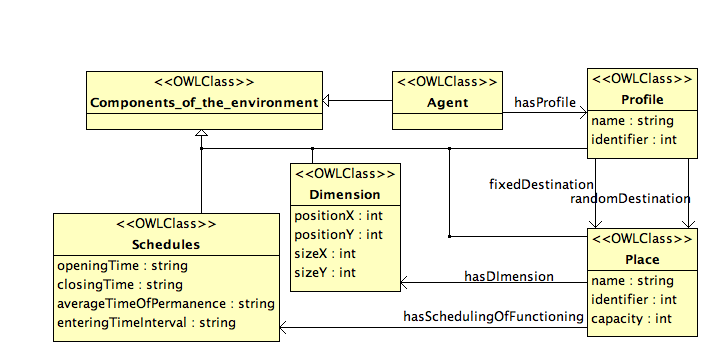
\includegraphics[width=150mm]{figuras/uem-tbox.png}
  \caption[T-Box baseado no modelo de ambiente urbano.]{T-Box baseado no modelo de ambiente urbano \cite{paiva2005ontology}.}
  \label{fig:UEM:TBOX}
\end{figure}

A Figura~\ref{fig:UEM:TBOX} demostra a ontologia, criada por
\citet{paiva2005ontology}, que será utilizada. As relações de generalização
possuem a mesma semântica que na UML, as relações direcionais são relações
binárias entre as instâncias das classes. Na figura, \emph{Agent} se relaciona
com o conceito \emph{Profile} para determinar o tipo de agente. O
\emph{Profile} do agente pode variar entre alguns tipos especificados pelo
usuário que podem possuir destinos fixos (usuais) ou destinos randômicos
(eventuais).

Esses locais são definidos pelo conceito \emph{Place} que contêm
uma descrição de sua capacidade (quantidade máxima de atores), dimensão
(acessível por relação) e horário de funcionamento (acessível por relação). O
conceito de \emph{Dimension} guarda a posição e o tamanho nos eixos X e Y. Já,
o conceito de \emph{Schedules} possui o horário de abertura e fechamento,
intervalo de entrada e tempo médio de permanência.

Além disso, o conceito \emph{Components\_of\_the\_environments} esta sendo
pensando como um sub-conceito de \emph{Setup} na ontologia
desenvolvida por causa que representa uma configuração.
%Essas configurações gerais são carregadas, normalmente, em outras partes do
%sistemas e então eliminadas por causa que elas não influenciam as emoções
%diretamente.
Fora isso, foi introduzida uma nova relação chamada \emph{hasCharacter} que
mapeia o conceito de agente da seção anterior para o conceito apresentado
aqui. Dessa forma, um agente na ontologia afetiva pode descobrir seu perfil e
seus locais visitados regularmente.

Essa ontologia é utilizada no presente trabalho de duas formas. A primeira
forma de utilização é para desenhar um mapa 2D do ambiente que os agentes
atuam. Isso é permitido porque o conceito \emph{Place} relaciona-se com o
\emph{Dimension}. Assim, todos os itens do mapa são retângulos. A outra forma
de utilização é a que trouxe a ontologia para o trabalho e é definir que um
agente tenha sua rotina descrita e disponibilizada pelo ambiente via
percepção. No ambiente simulado construído cada dia simulado equivale a
aproximadamente 96 ciclos, portanto, cada passo simulado equivale à em torno
de 15 minutos de um dia. Dessa forma, o ambiente é responsável por conhecer
que dia é e informar para cada agente sobre sua rotina do dia.

\section{Ontologia de Preferências} \label{ch:aec:oda}

\citet{doyle1998annotated} propuseram que o mundo contivesse uma série de
anotações nos objetos. Assim, o agente poderia conhecer apenas a forma de
questionar os objetos sobre suas formas de usar, suas descrições e suas outras
características. Esse conceito veio do conceito \emph{affordance} que se
refere a propriedade de um objeto que dita como o mesmo será utilizado.
Dessa forma, uma cadeira tem a propriedade de ser sentada e uma porta tem as
propriedades de ser aberta ou ser fechada.

Assim, eles utilizaram 5 tipos de anotações: (i) anotações emocionais,
explicam como um agente responde ``emocionalmente''; (ii) anotações de
resposta, explicam como o agente deve reagir ao evento no ambiente que pode ser
uma ação especifica ou uma sugestão de crença; (iii) anotações de resolução de
problemas, descreve o estado do problema e permite anotar dicas que o ator
talvez fale ou realize; (iv) anotações de papel, informam o agente sobre ações
relevantes para determinados trabalhos no mundo; (v) anotações de jogo,
descrevem o estado do jogo permitindo sugerir movimentos.

\citet{kallmann1999modeling} explicaram uma ideia similar, os objetos no mundo
são os responsáveis por proverem para o personagem o como ele deve ser usado.
Por exemplo, durante a animação do personagem estar abrindo uma porta, quem esta
no controle do ator é o ``agente'' que controla a porta. Sendo assim, o agente do
personagem delega a responsabilidade da animação para o agente do objeto por
causa que o mesmo é o único que sabe como realizar a animação de abertura ou
fechamento da porta. Esses objetos foram denominados objetos inteligentes e precisam
ter um determinado nível de conhecimento sobre o ator.

De uma maneira similar, o conceito de artefatos que possuem propriedades
observáveis e utilizáveis foi criado por \citet{ricci31cartago}. Por exemplo,
uma porta pode ter como propriedade observável seu estado (estar aberta ou
estar fechada) e ação possível ou propriedade utilizável ser aberta ou ser
fechada. Essas ações podem ficar disponíveis conforme o estado atual do
objeto, mas o controle da disponibilidade e da ação é do próprio objeto por
que é ele que sabe como realizar a ação propriamente dita. O agente unicamente
diz de alguma forma que o objeto tem que realizar tal ação. Nesse trabalho,
não é mencionado que o agente pode ser temporariamente controlado por
objetos.

\begin{figure}
  \centering
    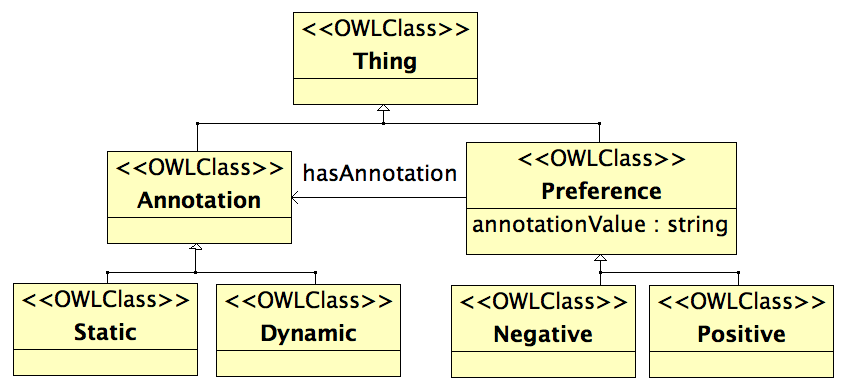
\includegraphics[width=130mm]{figuras/preferences.png}
  \caption{T-Box da ontologia de preferências proposta.}
  \label{fig:preferences}
\end{figure}

A ontologia proposta para as preferências pode ser vista na
Figura~\ref{fig:preferences}. Como pode ser observado, foi criado dois
conceitos principais \emph{Annotation} e \emph{Preference}. O conceito
\emph{Annotation} é utilizado para representar características de objetos.
Essas características podem ainda ser categorizadas entre as que mudam
e não mudam durante a simulação. O sub-conceito \emph{Dynamic} representa as
características dinâmicas, isto é, as características que podem ser alteradas
durante a ``vida'' do objeto. O sub-conceito \emph{Static} representa as
características que não podem ser alteradas depois da criação do objeto. O
calor e o dono são exemplos de características dinâmicas, enquanto o nome e a
capacidade total são exemplos de características estáticas.

O conceito \emph{Preference} é usado para representar as preferências por
determinadas características ou anotações. A preferência define como uma entidade ou
agente é atraído por determinada característica, por exemplo algumas pessoas
gostam de calor e outras não. Assim, as pessoas que gostam de calor são
atraídas pela valoração positiva da anotação de calor. Já, as pessoas que não
gostam de calor são atraídas pela valoração negativa. Dessa forma, os
sub-conceitos da preferência representam sempre valores que fazem o agente ser
atraído pelo objeto e repelido caso contrário.

Entretanto, esse exemplo não funciona para todos os casos. Por exemplo, um
agente tem conhecimento de seu nível de energia e este é sempre positivo. Para
resolver esse problema foi criada a relação \emph{hasAnnotationValue}
representada na Figura~\ref{fig:preferences} pelo atributo
\emph{annotationValue}. Sendo assim, é possível descrever que um agente com
nível de energia abaixo de um determinado limite é atraído pelo seu centro de
controle.

Essas anotações foram planejadas para serem colocadas pelo ambiente
nos objetos e nos agentes. As anotações em agentes permitem que os outros saibam
o que o agente esta fazendo e como ele parece de forma similar aos objetos. As
preferências também são disponibilizadas em formas de percepção, mas o usuário
que deve criar regras ou planos no \jason para montar as relações usadas pela
afetividade.

\section{Integrando a Plataforma \jason com as ontologias} \label{ch:p:ipjo}

As ontologias explicadas, nas seções anteriores, foram planejadas para serem
usadas como módulos. Sendo assim, as ontologias explicadas anteriormente
podem ser usada sem implicar no uso das demais. Cabe salientar que elas podem ser
usadas tanto pelo agente quanto pelo ambiente conforme poderá ser visto no
capítulo~~\ref{ch:cdu}.

\begin{figure}[b]
  \centering
  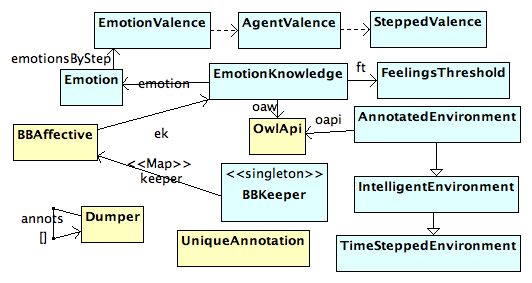
\includegraphics[width=8cm]{figuras/implementacao-15dez2011.png}
  \caption{Diagrama de classes do sistema.}
  \label{fig:dcs}
\end{figure}

Na figura~\ref{fig:dcs} pode ser observado as classes desenvolvidas para
realizar a integração das ontologias com os agentes \jason e o suporte
afetivo. Para essas classes serem usadas, o agente deve ser configurado para
utilizar a classe \emph{BBAffective} como base de crença. Essa configuração
pode ser feita conforme explicado na seção~\ref{sec-jason-architecture}
(pág.~\pageref{sec-jason-architecture}) e demostrado na seção~\ref{ch:cdu:tbc}
(pág.~\pageref{ch:cdu:tbc}). A classe \emph{UniqueAnnotation} é a responsável
por garantir a não duplicidade de anotações em percepções. %Assim, quando se
%insere por algum motivo duas vezes a mesma anotação apenas valerá a última.

A responsabilidade da classe \emph{BBAffective} é manter as crenças dos
agentes e atender as solicitações da plataforma \jason sobre a manipulação
dessas em dois níveis. O primeiro nível é a ontologia e o segundo é a base de
crença padrão que é utilizada quando o elemento não é considerado relevante
para o primeiro nível. A relevância é descoberta consultando os conceitos e
propriedades existentes na ontologia, por exemplo instâncias de conceitos são
crenças no formato ``nomeDoConceito(nomeDaInstancia)'' e relações são
similares à ``nomeDaRelacao(nomeDaInstanciaDominio, Imagem)''. Conhecer o que
é relevante para a ontologia é necessário porque a mesma é lenta e quanto
menos elementos contiver nela melhor será seu desempenho.

A base de crenças delega todo o assunto relacionado com as crenças da
ontologia para a classe \emph{EmotionKnowledge}. Essa é responsável por
conhecer todo o assunto relacionado com as emoções e sentimentos, porém ela
delega o conhecimento da história da potência das emoções para a classe
\emph{Emotion} e o conhecimento dos limites de ativação para a
\emph{FeelingsThreshold}. Da mesma forma, a manipulação e consulta da
ontologia, propriamente dita, é de responsabilidade da classe \emph{OwlApi}.

A classe \emph{Emotion} é responsável por conhecer todas as emoções presentes
e seus valores de potência. Para isso, no inicio da simulação a ontologia é
consultada procurando por todas as classes definidas\footnote{As classes
definidas possuem condições necessárias e suficientes, isto é, qualquer
indivíduo pode ser enquadrado nessa classe desde que obedeça as condições
suficientes.} sobre o conceito ``Emotion''. Isso é utilizado pela classe
\emph{EmotionKnowledge} quando a mesma precisa consultar o nome de uma emoção
por algum motivo. Por exemplo, na hora de calcular a valência da emoção em um
determinado passo é pedido pelo nome de todas as emoções à essa classe. Essa
ainda mantém a história da potência das emoções por agente para cada ciclo
armazenado utilizando um objeto da classe \emph{EmotionValence} que é um
extensão da classe \emph{HashMap} do \emph{Java}.

Para o suporte emotivo funcionar, a classe \emph{FeelingsThreshold} precisa
retornar que todos os limites mínimos de ativação dos sentimentos estão configurados.
Assim, ela é responsável por fazer essa verificação e por disponibilizar esses
limites para quando for realizado o cálculo da valência. Esse cálculo é
coordenado pela \emph{EmotionKnowledge} que consulta a ontologia, via instância
da classe \emph{OwlApi}, procurando as relações numéricas de cada indivíduo
que representa uma avaliação. Dessa forma, a potência é a soma de todas as
propriedades numéricas de um mesmo indivíduo.

As classes de ambiente, isto é, as classes que possuem \emph{Environment} no
nome são responsáveis por diversas coisas relacionadas com o ambiente. Por
exemplo, manter os passos de simulação com um tempo máximo, conhecer a
quantidade de agentes que tem que esperar responderem para ir ao passo de
simulação seguinte, carregar as ações definidas pelo usuário a partir de um
determinado pacote especificado e etc. Cabe salientar, as ações definidas no
ambiente precisam estender a classe \emph{EnvironmentAction} (não desenhada) e
estarem no pacote especificado na chamada a função ``loadAllActions''.

A classe \emph{Dumper} é responsável por conhecer o formato das crenças \jason
e converte-lo para um formato interno. Isso é necessário para proteger o
código feito de mudanças que a plataforma venha a ter. Assim, essa classe é
utilizada por todas as classes internas do sistema e, principalmente, pela
\emph{BBAffective} após constatada a relevância do elemento. Algumas funções
são, por exemplo, devolver os parâmetros do literal como \emph{string} ou número,
retornar uma instância de seu tipo a partir de um literal, criar o literal a
partir de uma \emph{string} ou a partir de uma outra instância de seu tipo e,
até mesmo, realizar a criação de um \emph{XML} para transferir os dados para
à ontologia.

Já, a classe \emph{BBKeeper} serve para facilitar o acesso a base de crenças.
Essa classe é a única \emph{singleton} do sistema e cada instância da
\emph{BBAffective} é conhecida por esta a partir do nome de seu respectivo
agente. Isso é muito útil para os exemplos porque torna possível acessar a
base de crenças e exibir os valores de potência e valência ou conhecer os
tipos emotivos disponíveis. Cabe salientar que os tipos emotivos disponíveis
do simulador não levam em conta o agente e, por isso, mesmo que seja usado um
agente que não esteja utilizando a base estendida os tipos serão retornados
corretamente.

As seções seguintes, explicam os novos processos de inserção, remoção,
consulta e listagem das crenças. Exemplos desses em código \emph{AgentSpeak}
são, respectivamente, \emph{+crencca}, \emph{-crencca}, \emph{?crencca} e
\emph{?X}. A listagem, também, é utilizada pela tela de visualização de
crenças quando realizando uma depuração no agente.

\subsection{Processo de Listagem e Consulta de Crenças}

\begin{figure}
  \centering
  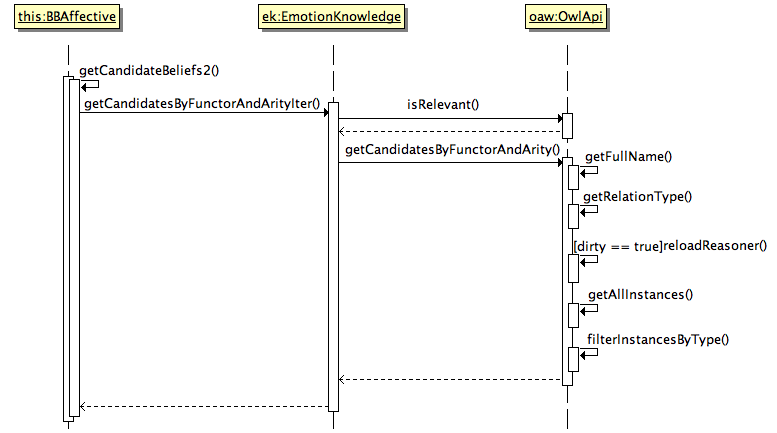
\includegraphics[width=12cm]{figuras/sd-getCB.png}
  \caption{Diagrama de sequência para consultar uma crença.}
  \label{fig:getCandidates}
\end{figure}

O processo de listagem serve para exibir todas as crenças e percepções do
agente. Isso é importante em momentos de depuração ou em momentos que se
deseja consultar uma crença que é uma variável não unificada, isto é, sem
valor definido. Dessa forma, a base de crenças implementa a interface
\emph{java.lang.Iterable} que permite a classe ser usada em construções
\emph{for-each}. A implementação devolve todos os elementos dos dois níveis
sendo que o nível da ontologia é recuperado primeiro.

De maneira similar, o processo de consulta de crenças foi alterado.
%Entretanto, ele pode ser chamado via código \jason ou pelo código \emph{Java}.
Esse processo tem como entrada os métodos com nome \emph{getCandidateBeliefs}
que chamam um método denominado \emph{getCandidateBeliefs2} conforme
pode ser visto na Figura~\ref{fig:getCandidates}. O resultado dessa operação é
um objeto \emph{Iterator} com todas as crenças recuperadas da base que possuem
o mesmo nome e mesma aridade que a informada na chamada. Isso é importante
porque esses candidatos podem ter seus parâmetros verificados pela própria
base de crenças ou por outros pontos de acesso do \emph{Jason}.

\subsection{Processo de Recuperação de Crenças}

O processo de recuperação de uma crença é necessário para a compreensão das
inserções e remoções de crenças. Ele serve para recuperar uma única crença
quando ela já existir na base, e em sua busca leva em consideração toda a
estrutura do literal excluindo às anotações. O procedimento é mostrado na
Figura~\ref{fig:recover}.

A recuperação é iniciada pela chamada do método \emph{contains}. Essa função
inicia com uma chamada à \emph{getCandidateBeliefs} que foi explicada na seção anterior.
Cada um dos candidatos retornados pela chamada são verificados para ver se
conferem com o informado pelo cliente, se conferir então o candidato é
retornado. Se nenhum candidato for retornado, o resultado da base de crenças
padrão será retornado porque o mesmo pode estar localizado neste nível.
Conforme foi falado anteriormente, tanto a inserção e remoção utilizam esse
procedimento para recuperar o elemento armazenado na base de crença, porém os
motivos serão vistos em suas respectivas seções.

\begin{figure}
  \centering
  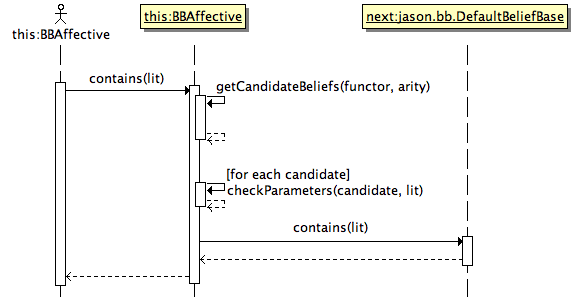
\includegraphics[width=100mm]{figuras/sd-contains.png}
  \caption{Diagrama de sequência para recuperar uma crença.}
  \label{fig:recover}
\end{figure}

\subsection{Processo de Adição de Crenças}

O procedimento de inserção de uma crença pode ser visto na
figura~\ref{fig:addBelief}. Essa figura utiliza as guardas do UML que são
etiquetas com o texto entre colchetes para informar a condição que o código
deve ter para ser executado. Além disso, elas encontram-se localizadas perto de
um quadrado para simbolizar que todas as chamadas feitas dentro deste estão
relacionadas aquelas condições. Dessa forma, quando estiver sendo inserida uma
crença de percepção com o termo diferente de ``step'' nenhum código será
executado pelo diagrama e a mesma será inserida no segundo nível.

A chamada do \jason para a função \emph{add} não se encontra representada na
figura~\ref{fig:addBelief}, porém essa função chama uma outra de mesmo nome e
quando essa retorna falso é chamada a função \emph{add} da instância
\emph{next}. Cabe chamar atenção que o processo de sumarização que calcula e
guarda a potência da emoção na classe \emph{Emotion} é realizado quando uma
percepção esta sendo inserida e o termo da crença é ``step''. Sendo assim, se
aproveita o momento para obter e inserir as percepções sobre os sentimentos
que acabaram de serem atualizados.

\begin{figure}
  \centering
  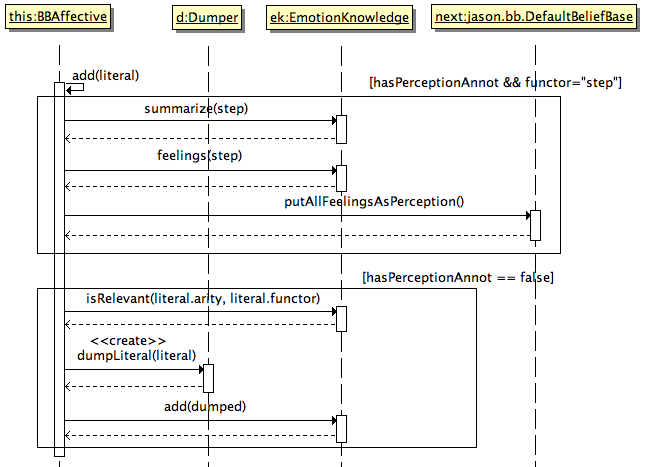
\includegraphics[width=12cm]{figuras/addB.png}
  \caption{Diagrama de sequência para adicionar uma crença.}
  \label{fig:addBelief}
\end{figure}

Agora quando esta sendo feita uma inserção de uma crença que não é uma
percepção, é feita a verificação se ele é relevante. Caso ele seja considerado
irrelevante, a crença sera inserida no segundo nível. Entretanto, se ele for
considerado relevante então será feita a recuperação do elemento atualmente
armazenado e, após isso, é feita a inserção das novas anotações nesse
elemento. Se o elemento não existir na base de crenças então esse último
procedimento é ignorado, porém ele é necessário para haver a correta
atualização das anotações. Por fim, a crença é transformada no tipo interno e
enviado para ser acrescentado na ontologia.

Assim, o processo de inserção serve para inserir os axiomas necessários para
representar essa crença na ontologia quando a mesma for relevante. Para a
criação na ontologia, é necessário ainda diferenciar se é uma instância de
objeto ou propriedade de dados ou de objetos. Essa diferenciação é feita pela
aridade e, em caso de ambiguidade, se pergunta o tipo à ontologia usando o
nome da entidade. A chamada \emph{Add} presente na Figura~\ref{fig:addBelief}
é explicada adiante.

\vfill

\subsection{Processo de Remoção de Crenças}

O processo de remoção de crenças permite remover uma crença da base de crenças
ou, apenas, atualiza-la retirando alguma anotação que não devia existir. Dessa
forma, o procedimento ao final do mesmo remove os axiomas postos anteriormente
e quando for uma atualização os insere novamente. A Figura~\ref{fig:delBelief}
mostra a rotina da base de crenças.

\begin{figure}
  \centering
  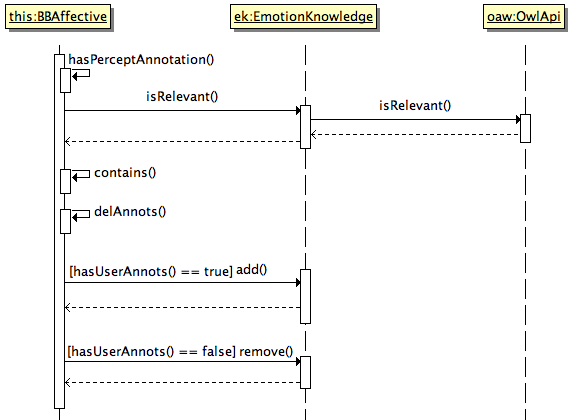
\includegraphics[width=10cm]{figuras/delB.png}
  \caption{Diagrama de sequência para remover uma crença.}
  \label{fig:delBelief}
\end{figure}

A rotina de remoção desenvolvida, inicia verificando se o termo é
considerado relevante. Se ele for uma percepção então ele é irrelevante para
esse procedimento. Caso não seja uma percepção, a relevância é verificada e
a sua relevância é constatada então o elemento armazenado é recuperado. Se não for
recuperado nenhum elemento ou se ele for irrelevante então é realizada a
chamada a remoção da base de crenças padrão e retornado o resultado.

Nesse momento o que se sabe é qual é a crença e que a mesma é relevante.
Assim, as anotações informadas são removidas da crença obtida e a nova
crença é testada para ver se ainda possui anotações. Se possuir e não for uma
anotação de fonte e não é um indicativo de estar sendo armazenada em
determinada ontologia então é feita a atualização do valor armazenado. No caso
de não possuir anotação ou possuir somente as anotações mencionadas é feita a
remoção do elemento. Tanto as funções \emph{Add} e \emph{Remove} da
Figura~\ref{fig:delBelief} compartilham o mesmo código e estão explicadas na
seção seguinte.

\subsection{Processo Compartilhado de Remoção e Adição de Crenças}

O processo de adição e remoção de crenças compartilham pedaços de códigos. A
classe \emph{EmotionKnowledge} possui dois pontos de entrada para adicionar ou
remover crenças, um pelo método \emph{Add} e outro pelo método \emph{Remove}.
Tanto um método quanto outro fazem uma chamada para uma função denominada
\emph{changeBelief} informando se o
procedimento é de inserção ou remoção. A partir dai a sequência de chamadas
mostradas na Figura~\ref{fig:shareBelief} segue de maneira igual. Isso foi
feito porque muito código é igual para ambos os casos.

\begin{figure}
  \centering
  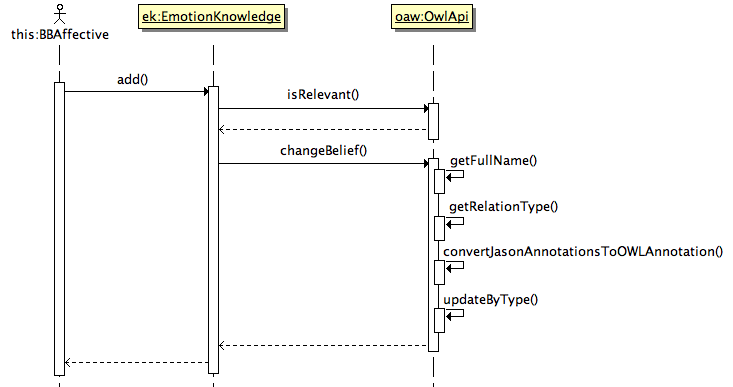
\includegraphics[width=12cm]{figuras/shareBelief.png}
  \caption{Diagrama de sequência para adicionar uma crença.}
  \label{fig:shareBelief}
\end{figure}

A classe \emph{OwlApi} é a única que consulta a ontologia diretamente via
biblioteca. No inicio da aplicação são extraídas as informações de quais
conceitos existem, quais relações e de que tipos elas são. Sendo assim,
consultar o nome completo de uma determinada entidade ou qual é seu tipo não
precisa ir na ontologia. A função \emph{updateByType} é a responsável por
realizar a inserção e remoção dos axiomas. Uma alteração é feita removendo
os axiomas anteriores, acrescentando os novos e marcando a ontologia como suja
para quando uma consulta for feita a mesma ter o raciocinador atualizado.

